Full details for all scripts, including all required dependencies, are in the \lref{https://github.ncsu.edu/MakerSpaceControl/RaspberryPiBuild/blob/main/README.md}{README}.
A POSIX-like operating system is required for building the image and recommended for other the other steps.

\subsection{Building the Raspberry Pi Image}

\begin{subsubsec}{GitHub Deploy Keys}
    GitHub deploy keys are permission-restricted SSH keys for specific repositories.
    We use a read-only deploy key to download and update the software on each Raspberry Pi.
    A file at \textbf{\mintinline{bash}{$HOME/.ssh/access_key}} holds the credentials,
        and \textbf{\mintinline{bash}{$HOME/.ssh/config}} is set to use it.

    In the build script directory, \textbf{\mintinline{bash}{.access_key}} is copied into the image as a deploy key.
    If this is not in the directory (check with \textbf{\mintinline{bash}{ls -a}}),
        copy the file in to the directory.
    If you do not have access to an existing key, \lref{https://docs.github.com/en/authentication/connecting-to-github-with-ssh/generating-a-new-ssh-key-and-adding-it-to-the-ssh-agent}{generate one} and skip adding it to the ssh agent.
    Select ``Add deploy key'' in ``MakerSpaceControl/RaspberryPiSoftware'' $\rightarrow$ ``Settings'' $\rightarrow$ ``Deploy keys'' using the corresponding public key \cref{fig:add deploy key}.
    The public key is in \textbf{\mintinline{bash}{KEY_NAME.pub}}, i.e. \textbf{\mintinline{bash}{$HOME/.ssh/access_key}} has a public key at \textbf{\mintinline{bash}{$HOME/.ssh/access_key.pub}} after generation.

    To change deploy keys after build, mount the image file (\textbf{\mintinline{bash}{mount -o IMAGE.img MNT_DIR}}) or the SD card (\textbf{\mintinline{bash}{mount IMAGE_PARTITION MNT_DIR}}).
    Replace the key in the image (\textbf{\mintinline{bash}{cp KEY MNT_DIR/home/Project13/.ssh/access_key}}).
    Then unmount the image file or SD card (\textbf{\mintinline{bash}{umount MNT_DIR}}) before removing any media.
    
    \begin{figure}
        \centering
        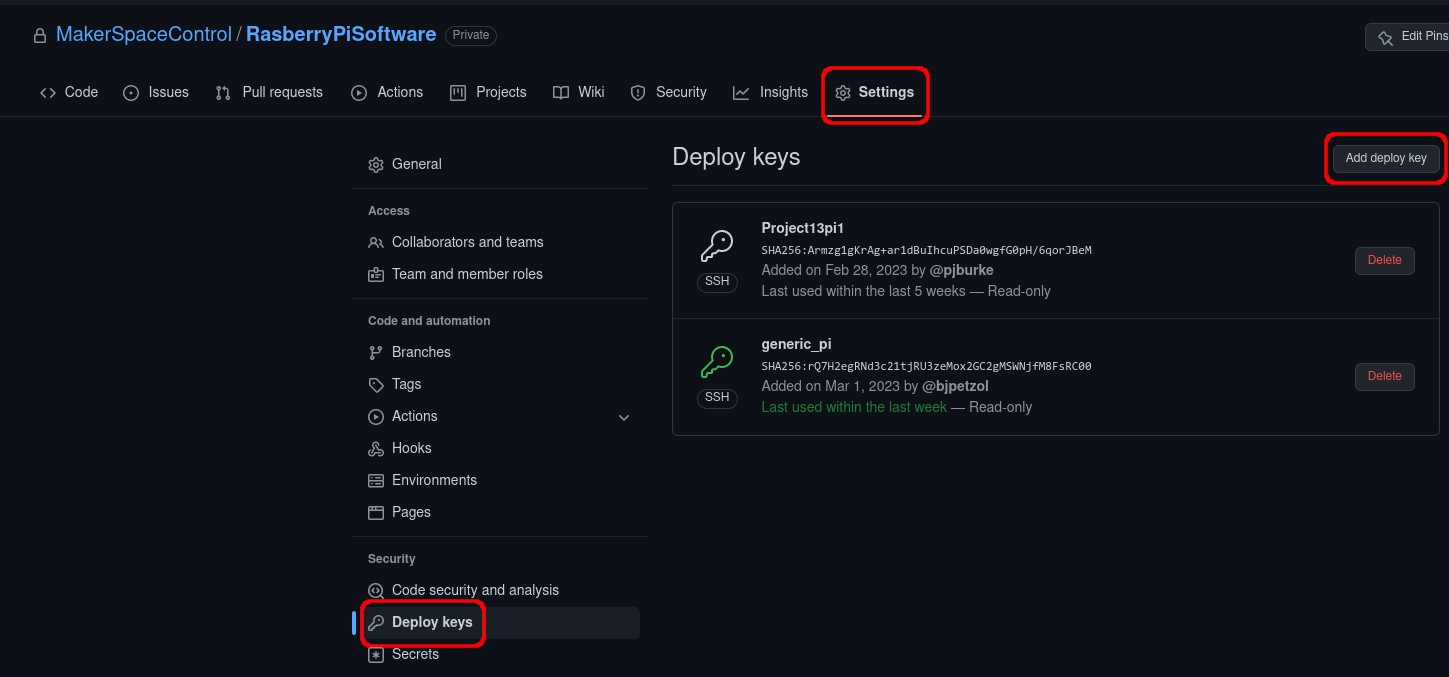
\includegraphics[width=\textwidth]{Deploy_Marked_Up.png}
        \caption{Adding a Deploy Key}
        \label{fig:add deploy key}
    \end{figure}
\end{subsubsec}

\begin{subsubsec}{User Settings}
    Two passwords are kept in the build script directory.
    The user password is in the plaintext \bashline{.password} and \bashline{.root_password} has the root password.
    All three identity files (\bashline{.password}, \bashline{.root_password}, and \bashline{.access_key}) are \emph{deliberately} ignored by git for security.
    These files need to be copied to any new image build directories.
\end{subsubsec}

\begin{subsubsec}{Running the Build Script}
    The build script is run with \bashline{./build.bash} and constructs an xz compressed image file.
    This script requires QEMU, sudo, and a user with sudo access to mount and build the image.
    Creating a new image takes at least half an hour,
        as the script needs to update and install many packages inside a virtual environment.
    The script needs to be given a superuser password after downloading a base image,
        but otherwise runs unattended.
    The output is tagged with the build date as per the build machine's clock.
\end{subsubsec}

\subsection{Updating the Image}
    The update script is run with \bashline{./update.bash IMAGE.img} and constructs a new xz compressed image without destroying the provided base image.
    This requires the same permissions and tools as the build script,
        but is significantly faster.
    The script updates the image to have the latest packages and MakerSpace control code.
    The output is tagged with the build date as per the build machine's clock.
    
\subsection{Flashing the Image}
    The image can be written to an SD card with \bashline{./install.bash IMAGE.img DISK...},
        which provides convenience progress displays and automatically expands every partition to maximum size.
    Other image writing tools, such as \lref{https://www.raspberrypi.com/software/}{Raspberry Pi Imager} or \lref{https://www.balena.io/etcher}{Balena Etcher} can also decompress and write the file with progress information.
    If using a third-party tool,
        this step does not require a POSIX-like machine.
    Make sure the SD card is fully written to before removing it.
    The tools should wait for a full write before showing as complete,
        but this can be verified on a POSIX-like machine by running \\
        \hspace*{2em} \bashline{for device in /sys/block/*; do awk '{ print "$device: "  $9 }' "${device}/stat"} \\
        and confirming that all sdX devices have a ``0'' status.

\subsection{First Machine Boot}
    Once the SD card is written,
        it can be placed in the slot of the target Raspberry Pi.
    Assemble it with the rest of the physical system [\cref{sec: final-assembly}] and connect it to both ethernet and power.
    When the module is first powered on,
        and only when it is first powered on,
    it will display a MAC address for 30 seconds after booting.
    This MAC address is used as an identifier for management and communications with the remote server.
    Note it down and add the MAC address to the system.
    When the MAC address is added to the management database,
        the module will finish configuring itself and be fully functional without a reboot.
